\section{Theorie}
\label{sec:Theorie}

Zunächst wird allgemein auf Polarisation von Wellen eingegangen.
Dann wird sich mit dem prinzipiellen Aufbau eines Lasers beschäftigt und wie dieser kohärentes Licht produziert.
Außerdem wird behandelt, was unter TEM-Moden verstanden wird.
Schließlich wird konkret der klassische Aufbau eines Helium-Neon-Lasers und dessen Eigenschaften behandelt.

\subsection{Polarisation und Kohärenz} \label{sec:polarisation}
Seit der Elektrodynamik ist bekannt, dass Licht als eine elektromagnetische Welle beschrieben werden kann.
\textbf{Kohärentes Licht} beschreibt Licht mit fester Frequenz, Phase und Ausbreitungsrichtung und kann mithilfe von Lasern erzeugt werden.
Nun ist bei verschiedenen physikalischen Prozessen auch die sogenannte \textbf{Polarisation} wichtig.
Eine polarisierte Welle ist in \autoref{fig:polarisation1} dargestellt.
Eine polarisierte Welle schwingt nur in einer Ebene in Bewegungsrichtung.
Beispielweise bei Interferenzphänomenen müssen zwei Lichtwellen in einer Ebene polarisiert sein, damit sie interferieren können.
\begin{figure}
    \centering
    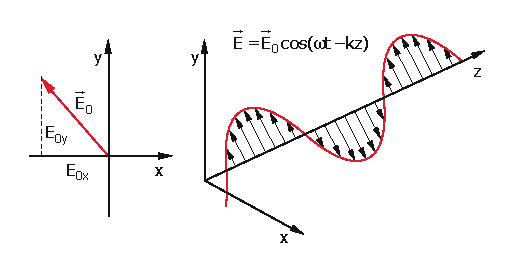
\includegraphics[width = 0.7 \linewidth]{pictures/polarisation1.pdf}
    \caption{Eine linear polarisierte Welle \cite{demtroeder2}.}
    \label{fig:polarisation1}
\end{figure}
\subsection{Aufbau eines Lasers}
\label{sec:aufbau1} 
\begin{figure}
    \centering
    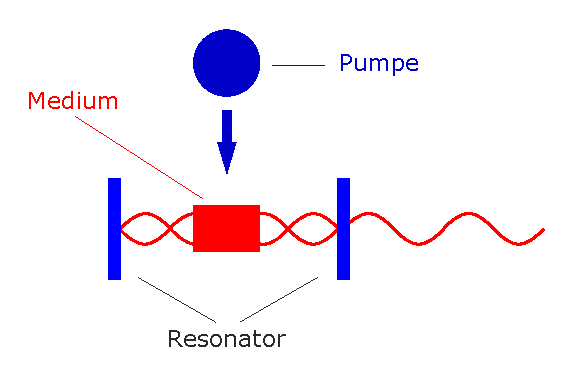
\includegraphics[width = 0.7 \linewidth]{pictures/aufbau1.pdf}
    \caption{Schematischer Aufbau eines Lasers \cite{leifilaser}.}
    \label{fig:aufbau1}
\end{figure}
Wie bereits angemerkt, produziert ein Laser (Light Amplification by Stimulated Emission of Radiation) kohärentes Licht.
Im folgenden soll darauf eingegangen werden wie kohärentes Licht in einem Laser produziert wird.
Schematisch ist der Aufbau eines Lasers in \autoref{fig:aufbau1} dargestellt.
Grundlegend besteht ein Laser immer aus drei Komponenten.
Diese Komponenten sind ein sogenanntes \textbf{aktives Medium}, ein \textbf{Resonator} und eine \textbf{Pumpquelle}.
\subsubsection*{Aktives Medium}
\begin{wrapfigure}{r}{0.5\textwidth}
    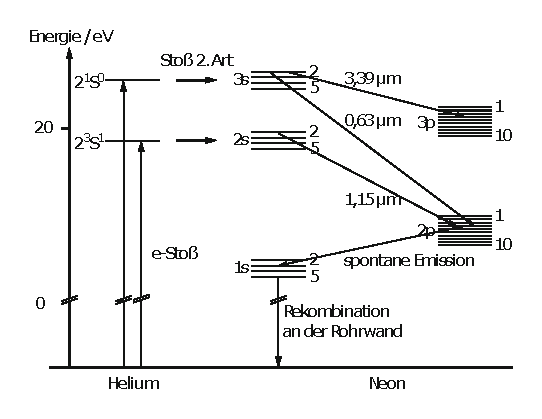
\includegraphics[width=0.8\linewidth]{pictures/HeNe_levels.pdf}
    \caption{Der Ablauf der Emission eines Photons bei einem HeNe-Laser \cite{HeNe_levels}.}
    \label{fig:HeNe_levels}
\end{wrapfigure}
Unter einem aktiven Medium wird verstanden, dass es durch \textbf{Besetzungsinversion} und \textbf{stimulierter Emission} kohärentes Licht abgibt \cite{demtroeder_laser}.
Eingeleitet wird dies dadurch, dass Photonen durch spontane Emission freigesetzt werden und dann verstärkt werden.
In einem Laser wird dies dann so angeordnet, dass es immer weiter verstärkt wird (Resonator).
Ein Material ist dann ein geeigneter Kandidat für ein aktives Medium, wenn es über ein 3-Niveau-System\footnote{Aufgrund der Notwendigkeit eines metastabilen Zwischenzustandes, ist ein 2-Niveau-System nicht möglich.} verfügt.
Dann lässt sich mit der stimulierten Emission die Abstrahlung des Photons bei Anregung verstärken.
Dies geschieht dadurch, dass das angeregte Photon mit einem weiteren Photon angestrahlt wird und dann durch quantenmechanische Effekte beim Abstrahlen quasi kopiert wird (kohärent).
Durch die stimulierte Emission und den Resonator kommt es dann zu der Besetzungsinversion.
Dabei befinden sich dann mehr Elektronen in einem höheren Energiezustand als im Grundzustand.
Das Medium kann dabei fest, flüssig oder auch gasförmig sein.
Weiterhin legt das aktive Medium auch die Wellenlänge des Lasers fest, da es sich dabei um das charakteristische Spektrum des Mediums handelt.

\subsubsection*{Resonator}
Der Resonator besteht im Grunde aus zwei Spiegeln.
Einer davon ist teildurchlässig. Dabei handelt es sich um die Seite, die als Öffnung bei einem Laser bekannt ist.
Dadurch bleiben statistisch gesehen immer einige Lichtwellen im Resonator und können durch stimulierte Emission das kohärente Licht immer weiter verstärken.
Ohne den Resonator würde sich das Licht willkürlich in alle Richtungen ausbreiten und es nicht zur Besetzungsinversion kommen und sich kein Lichtstrahl ausbilden.
Weiterhin lässt sich die Resonatorstabilität mit den sogenannten g-Faktoren 
\begin{equation} \label{eq:gfaktor}
    g_i = 1 - \frac{L}{r_i}
\end{equation}
beschreiben. Dabei ist $r_i$ der Krümmungsradius und $L$ die Länge des Resonators.
Für $0 < g_1 g_2 < 1$ ist der Resonator stabil.
Daraus lässt sich auch der maximale Abstand zwischen den Spiegeln berechnen.
Bei zwei gleichen Spiegeln wird dieser immer dann kleiner null, wenn er größer als der Krümmungsradius ist.

\begin{wrapfigure}{r}{0.4\linewidth}
    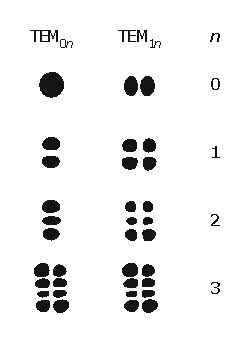
\includegraphics[width=\linewidth]{pictures/moden1.pdf}
    \caption{$TEM_{xy}$ \cite{HeNe_levels}.}
    \label{fig:moden1}
\end{wrapfigure}
Der Name Resonator lässt bereits darauf schließen, dass sich stehende Wellen innerhalb des Resonators ausbilden.
Dabei können longitudinale und transversale Moden entstehen.
Die longitudinalen Moden sind bei Aufbauten wie in \autoref{fig:aufbau2} nicht relevant, da die Wellenlänge der emittierten Strahlung deutlich geringer ist als die Länge des Resonators.
Die transversalen elektromagnetischen Moden ($TEM_{xy}$) sind jedoch deutlich relevanter.
Die $TEM_{xy}$ bezeichnen die Anzahl der Knoten auf der entsprechenden Achse.
Beispielhaft wurden einige in \autoref{fig:moden1} aufgezeichnet.
Es gibt auch den Fall, dass die Moden zylindrisch sind.
In diesem Fall gilt $TEM = TEM_{\phi r}$.
Hier nimmt die Intensität der Moden nach außen hin immer weiter ab.
Ohne weitere Herleitung sei angegeben \cite{demtroeder_laser}, dass die Intensität bei einer $TEM_{00}$ Mode durch
\begin{equation} \label{eq:tem00}
    I  =I_0 e^{- \frac{2 r^2}{\omega^2}}
\end{equation}
gegeben ist. Dabei ist $\omega$ der Strahlradius.
Für die $TEM_{01}$ Mode ergibt sich eine Intensität von
\begin{equation} \label{eq:tem01}
    I  =I_0 \cdot \left( \frac{r}{\omega} \right)^2 \cdot e^{- \frac{2 r^2}{\omega^2}} \, .
\end{equation}

\subsubsection*{Pumpquelle}
Die Pumpquelle ist in erster Linie dafür verantwortlich, Energie in das aktive Medium zu bringen.
Dies kann durch Licht, aber auch durch andere Prozesse geschehen.
Ohne dieses Pumpen, kann keine Besetzungsinversion vorliegen.

\subsection{Der HeNe-Laser}
\begin{figure}
    \centering
    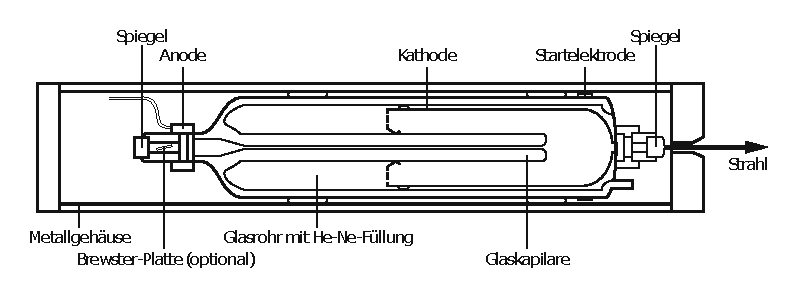
\includegraphics[width = 0.7 \linewidth]{pictures/aufbau2.pdf}
    \caption{Schematischer Aufbau eines HeNe-Lasers \cite{HeNe_levels}.}
    \label{fig:aufbau2}
\end{figure}
Der Aufbau eines HeNe-Lasers ist in \autoref{fig:aufbau2} zu sehen.
Die Niveaus, die in einem HeNe Laser durchlaufen werden, sind in \autoref{fig:HeNe_levels} dargestellt.
Bei einem Helium-Neon Laser (HeNe) liegt diese Wellenlänge bei $632.8 \unit{\nano\meter}$.
Dies lässt sich aber auch verändern, je nachdem welche Art von selektiven Spiegeln verbaut werden.
Diese lassen dann im Resonator einige Wellen ungehindert durch.
Durch diese Art von Spiegeln lässt sich bei HeNe-Laser auch orange, gelbe und grüne Strahlen erzeugen. 
Als weiteres Bauteil sind die Brewster-Fenster verbaut.
Die Brewster-Fenster zeichnen sich dadurch aus, dass sie parallel zur Einfallsebene polarisiertes Licht verlustfrei hindurchlassen.
Das Licht trifft im Brewster-Winkel auf.
Für senkrecht polarisiertes Licht ist das Reflexionsvermögen allerdings sehr hoch, weshalb dieses Licht im Laser unterdrückt wird.
Die Intensität in Abhängigkeit von dem Winkel wird beschrieben durch das Gesetz von Malus, also
\begin{equation} \label{eq:malus}
    I(\alpha) = I_0 \cdot \cos^2(\alpha) \, .
\end{equation}